%-------------------------------------------------------------------------------
%-------------------------------------------------------------------------------
%-------------------------------------------------------------------------------
\chapter{Couplages}
%-------------------------------------------------------------------------------
%-------------------------------------------------------------------------------
\thispagestyle{empty}
%-------------------------------------------------------------------------------
%-------------------------------------------------------------------------------
%-------------------------------------------------------------------------------
\section{Couplages généraux}
%-------------------------------------------------------------------------------
%-------------------------------------------------------------------------------
%-------------------------------------------------------------------------------

$G=(S,A)$ est un graphe non orienté, $S$ est l'ensemble de ses sommets, $A$ l'ensemble de ses arêtes.

On note $\sigma(a)$ l'ensemble des deux sommets reliés par une arête $a$.

On supposera que $G$ est sans point isolé : $\displaystyle \bigcup_{a \in A} \sigma(a)=S$.
%-------------------------------------------------------------------------------
%-------------------------------------------------------------------------------
\subsection{Recouvrement par les sommets}
%-------------------------------------------------------------------------------
%-------------------------------------------------------------------------------
Un {\bf stable} de $G$ est une partie $S'$ de $S$ ne contenant aucune paire de sommets adjacents : 
\[\forall a\in A\quad |\sigma(a)\cap S'| \le 1\]
Le cardinal maximum d'un stable de $G$ est noté $\alpha(G)$.

\smallskip

Un {\bf transversal} est une partie $T$ de $S$ contenant un sommet adjacent à toute arête :
\[\forall a\in A\quad |\sigma(a)\cap T| \ge 1\]
Le cardinal minimum d'un transversal de $G$ est noté $\beta(G)$.
%--------------------------------------------------------------------------
%--------------------------------------------------------------------------
\begin{Exercise}[title=Une première dualité]\it
Prouver les assertions suivantes.

\begin{enumerate}
\item $S'$ est un stable si et seulement si $S\setminus S'$ est un transversal.
\item $\alpha(G)+\beta(G)=|S|$
\end{enumerate}
\end{Exercise}
%--------------------------------------------------------------------------
\begin{Answer}
On note $\overline{S'} = S\setminus S'$ et $n = |S|$.
\begin{enumerate}
\item $\bigl|\sigma(a)\cap S'\bigr|+\bigl|\sigma(a)\cap \overline{S'}\bigr|
\bigl|\sigma(a)\cap S\bigr| = \bigl|\sigma(a)\bigr|=2$ donc

$\big[\forall a\in A\ \bigl|\sigma(a)\cap S'\bigr|\le 1 \bigr] \iff 
\bigr[\forall a\in A\bigl|\sigma(a)\cap \overline{S'}\bigr|\ge 1\bigr]$

\item Si $S'$ est un stable de cardinal maximal, $\alpha(G)$, alors $\overline{S'}$ est un recouvrement 

donc  $\beta(G) \le |\overline{S'}| = n - |S'|= n - \alpha(G)$ : $\alpha(G)+\beta(G) \le n$.

Si $T$ est un recouvrement de cardinal minimal, $\beta(G)$, alors $\overline T$ est un stable 

donc  $\alpha(G) \ge |\overline T| = n - |T| = n - \beta(G)$ : $\alpha(G)+\beta(G) \ge n$.

On a bien $\alpha(G)+\beta(G) \ge n$.
\end{enumerate}
\end{Answer}
%-------------------------------------------------------------------------------
%-------------------------------------------------------------------------------
\subsection{Recouvrement par les arêtes}
%-------------------------------------------------------------------------------
%-------------------------------------------------------------------------------
Un {\bf couplage} de $G$ est une partie $C$ de $A$ ne contenant aucune paire d'arêtes adjacentes : 
\[\forall a,a'\in C\quad \sigma(a)\cap \sigma(a')=\emptyset\]
Le cardinal maximum d'un couplage de $G$ est noté $\alpha'(G)$.

\smallskip

Un {\bf recouvrement} est une partie $R$ de $A$ contenant une arête adjacente à tout sommet : 
\[\sigma(R) := \bigcup_{a \in R} \sigma(a)=S\]
Le cardinal minimum d'un recouvrement de $G$ est noté $\beta'(G)$.
%--------------------------------------------------------------------------
%--------------------------------------------------------------------------
\begin{Exercise}[title=Comparaisons]\it 
Prouver qu'on a $2\alpha'(G) \le |S| \le 2\beta'(G)$.
\end{Exercise}
%--------------------------------------------------------------------------
\begin{Answer}

Pour un couplage $C$ les extrémités des arêtes sont distinctes donc $2|C| \le n$.

Pour un recouvrement $R$ tout sommet est l'une des deux extrémités des arêtes de $R$ donc $n \le |R|$.
\end{Answer}
%--------------------------------------------------------------------------
%--------------------------------------------------------------------------
\begin{Exercise}[title=Théorème de Gallai]\it 
\begin{enumerate}
\item Si $C$ est un couplage de cardinal maximal prouver que $S\setminus \sigma(C)$ est un stable.
\item Si $R$ est un recouvrement de cardinal minimal prouver que toute arête de $R$ admet au moins un sommet qui n'est adjacent qu'à une seule arête de $R$.
\item Prouver qu'on a $\alpha'(G)+\beta'(G)=|S|$
\end{enumerate}
\end{Exercise}
%--------------------------------------------------------------------------
\begin{Answer}
\begin{enumerate}
\item Soit $C$ un couplage. Si $\overline{\sigma(C)}$ n'est pas un stable, il existe une arête $a$ dont les deux extrémités sont dans $\overline{\sigma(C)}$ d'où $C \cup\{a\}$ est encore un couplage : $C$ n'est pas de cardinal maximal d'où le résultat par contraposition.

On a démontré en fait que si $C$ est un couplage maximal pour l'inclusion (ce qui est plus général que la maximalité du cardinal
\item Soit $R$ un recouvrement. S'il existe $a\in R$ dont les deux sommets sont adjacents chacun à une autre arête de $R$ alors $R\setminus\{a\}$ est encore un recouvrement donc $R$ n'est pas de cardinal minimal. Le résultat s'en déduit par contraposition.
\item Soit $C$ un couplage de cardinal maximal, les sommet du stable $S' = \overline{\sigma(C)}$ ne sont pas reliées par des arêtes mais ont chacun une arête adjacente car le graphe n'a pas de sommet isolé.

Si on ajoute ces arêtes à $C$ on obtient un recouvrement $R$ avec $|R| = |C| + |S'|$.

Or les arêtes de $C$ sont non adjacentes donc $|\sigma(C)| = 2|C|$ puis $|S'| = n - 2|\sigma(C)|
=2 -2|C|$ ; ainsi $|\beta'(G) \le |R| = n - |C| = n - \alpha'(G)$. On a $\alpha'(G)+\beta'(G)\le |S|$.

Soit $R$ un recouvrement de cardinal minimal. Pour chaque arête de $R$ on choisit un sommet qui n'est adjacent qu'à cette arête. Il reste $n - |C|$ sommets. On obtient un couplage en choisissant une arête de $R$ (il peut y en avoir plusieurs) pour chacun de ces sommets restants. On a ainsi
$\alpha'(G) \ge n - |C| = n - \beta'(G)$ d'où $\alpha'(G)+\beta'(G)\ge |S|$ puis l'égalité.
\end{enumerate}
\end{Answer}
%-------------------------------------------------------------------------------
%-------------------------------------------------------------------------------
\subsubsection{Couplages parfaits}
%-------------------------------------------------------------------------------
%-------------------------------------------------------------------------------
Un couplage est {\bf parfait} s'il est en même temps un recouvrement.
%--------------------------------------------------------------------------
%--------------------------------------------------------------------------
\begin{Exercise}[title=Un critère]\it 
Prouver que $G$ admet un couplage parfait si et seulement si $2\alpha'(G) = |S| = 2\beta'(G)$.
\end{Exercise}
%--------------------------------------------------------------------------
\begin{Answer}

Si $G$ admet un couplage parfait $C$ alors $|C|\le \alpha'(G)$ car $C$ est un couplage et $|C|\ge \beta'(G)$ car $C$ est un recouvrement. On a donc $2\alpha'(G) \ge 2\beta'(G)$, comme l'inégalité inverse est toujours vraie, on en d"duit $\alpha'(G) = \beta'(G)$. Comme la somme est égale à $n$ la valeur commune est $\frac n2$.

Inversement si $\alpha'(G) = \frac n2$ alors, pour un couplage $C$ de cardinal maximal, les sommets couverts forment un ensemble de cardinal $2|C| = n$ donc $C$ est aussi un recouvrement, c'est un couplage parfait.
\end{Answer}
%--------------------------------------------------------------------------
%--------------------------------------------------------------------------
\subsection{Augmentations}
%--------------------------------------------------------------------------
%--------------------------------------------------------------------------
$G$ est un graphe muni d'un couplage $C$.

Un sommet est couplé s'il appartient à $\sigma(a)$ pour une arête $a\in C$.

Une chaîne {\bf alternée} relativement au couplage est une suite finie de sommets distincts $(x_0,x_1,\ldots,x_p)$ telle que 
\begin{itemize}
  \item $x_0$ n'est pas couplé,
  \item $(x_{2k},x_{2k+1})$ est une arête de $G$ n'appartenant pas à $C$ 
  
  et $(x_{2k-1},x_{2k})$ appartient à $C$ pour tout $k\le n\div 2$.
\end{itemize}

\smallskip

Une chaîne alternée est {\bf augmentante} si, de plus, $x_n$ n'est pas couplé.

%--------------------------------------------------------------------------
\begin{Exercise}[title=Augmentation]\it 
Prouver que si un couplage $C$ admet une chaîne alternée augmentante $(x_0,x_1,\ldots,x_p)$ alors $p$ est impair et $C$ n'est pas de cardinal maximum.
\end{Exercise}
%--------------------------------------------------------------------------
\begin{Answer} 

Si $p$ était pair, $p\ge 2$ alors $p$ serait une extrémité de l'arête $(x_{p-1}, x_p)\in C$.
On pose $p = 2q + 1$.

On remplace les $q$ arêtes $(x_1, x_2)$, $(x_3, x_4)$, \dots, $(x_{2q-1}, x_{2q})$ par les 
$q+1$ arêtes $(x_0, x_1)$, $(x_2, x_3)$, \dots, $(x_{2q}, x_{2q+1})$ dans $C$. Le résultat est toujours un couplage, dont le cardinal est supérieur de 1 à celui de $C$.
\end{Answer}
%--------------------------------------------------------------------------
%--------------------------------------------------------------------------
\subsubsection{Différence ensembliste} 
%--------------------------------------------------------------------------
%--------------------------------------------------------------------------

Si $X$ et $Y$ sont deux ensembles leur {\bf différence ensembliste} est
\[X\Delta Y := (X\setminus Y) \cup (Y\setminus X) = (X\cup Y) \setminus (X\cap Y)\]

Si $C$ est un couplage et si $(x_0,x_1,\ldots,x_p)$ est une chaîne augmentante pour $C$, la preuve de l'exercice précédent consiste à prouver que $C \Delta \Gamma$ est toujours un couplage avec $\Gamma = \bigl\{(x_0, x_1), (x_2, x_2), \ldots, (x_{p-1}, x_p)\bigr\}$.
%--------------------------------------------------------------------------
%--------------------------------------------------------------------------
\begin{Exercise}[title=Existence de chaînes augmentantes]\it 
Si $C$ et $C$ sont deux couplages de $G$ avec $|C| < |C'|$, prouver que $C \Delta C'$ contient une chaîne augmentante pour $C$.
\end{Exercise}
%--------------------------------------------------------------------------
\begin{Answer}
Dans $C$ et dans $C'$ les arêtes n'ont pas de sommet en commun ; ainsi, dans $C \Delta C'$ un sommet ne peut être l'extrémité que de deux arêtes au plus (chaque sommet est de degré 2 au plus) et, dans le cas où deux arêtes ont un sommet commun, l'une appartient à $C$ et l'autre à $C'$.

On en déduit que les composantes connexes de $C \Delta C'$ sont
\begin{itemize}
    \item soit des chemins simples alternant les arêtes de $C$ et les arêtes de $C'$,
    \item soit des cycles de longueur paire.
\end{itemize}

\newpage

Les composantes connexes contiennent donc
\begin{itemize}
    \item soit autant d'arêtes de $C$ et d'arêtes de $C'$, c'est le cas des cycles car ils sont d'ordre pair,
    \item soit une arête de $C$ de plus que le nombre d'arêtes de $C'$, c'est donc un chemin qui commence et finit par une arête de $C$ : une chaîne alternée augmentante pour $C'$, 
    \item soit une arête de $C'$ de plus que le nombre d'arêtes de $C$, c'est donc un chemin qui commence et finit alors par une arête de $C'$ : une chaîne alternée augmentante pour $C$.
\end{itemize}


Si on note $n = |C|$, $n' = |C'|$ et $d = |C \cap C'|$, on a $n < n'$ et le nombre d'arêtes de $C$ (resp. de $C'$) dans $C \Delta C'$ est $n-d$ (resp. $n'-d$).

Il y a donc plus d'arêtes de $C'$ que d'arêtes de $C'$ dans $C \Delta C'$ ; d'après le décompte ci-dessus, on en déduit qu'il existe au moins $n'-n$ chaînes alternées augmentantes pour $C$ dans $C\Delta C'$.
\end{Answer}
%--------------------------------------------------------------------------
%--------------------------------------------------------------------------
\begin{Exercise}[title=Théorème de Berge]\it
Prouver qu'un couplage $C$ est de cardinal maximum si et seulement si il n'admet pas de chaîne alternée augmentante.
\end{Exercise}
%--------------------------------------------------------------------------
\begin{Answer}On a déjà vu la contraposée du sens direct : si un couplage admet une chaîne alternée augmentante, il n'est pas de cardinal maximal.

Inversement, si $C$ est un couplage non maximal, il existe un couplage $C'$ tel que $|C'| > |C|$ et la question précédente montre qu'il existe une chaîne alternée augmentante pour $C$ dans $C \Delta C'$.
\end{Answer}
%--------------------------------------------------------------------------
%--------------------------------------------------------------------------
%--------------------------------------------------------------------------
\section{Couplages dans les graphes bipartis}
%--------------------------------------------------------------------------
%--------------------------------------------------------------------------
%--------------------------------------------------------------------------
Un graphe non orienté $(S,A)$ est {\bf biparti} si l'ensemble des sommet peut s'écrire sous une forme d'union disjointe $S = U \sqcup V$ telle que toute arête ne peut joindre qu'un sommet de $U$ à un sommet de $V$ : $A \subset U \times V \cup V\times U$.

\medskip

Un graphe biparti est {\bf équilibré} si  $|U|=|V|$.

\newpage

Comme les chaînes alternées relativement à un couplage $C$ alternent aussi les sommets dans $U$ et $V$ et qu'une chaîne alternée augmentante a un nombre pair de sommets on en déduit que ses extrémités appartiennent l'une à $U$ et l'autre à $V$. On ne considérera ici que les chaînes alternées augmentantes d'origine dans $U$ et d'extrémité dans $V$.
\[x_0 \rightarrow x_1 \rightarrow x_2\rightarrow \cdots \rightarrow x_{p-1} \rightarrow x_p\]
\begin{itemize}
    \item $p$ est impair
    \item $x_i\in U$ pour $i$ pair, $x_i\in V$ pour $i$ impair, 
    \item $(x_i, x_{i+1})\notin C$ pour $i$ pair, $(x_i, x_{i+1})\in C$ pour $i$ impair. 
\end{itemize}
%--------------------------------------------------------------------------
%--------------------------------------------------------------------------
\subsection{Dénombrements}
%--------------------------------------------------------------------------
%--------------------------------------------------------------------------

$C$ est un couplage d'un graphe biparti $(U\sqcup V, A)$.

\begin{itemize}
    \item $U_0$ est l'ensemble (éventuellement vide) des sommets de $U$ qui ne sont pas extrémité d'une arête de $C$.
    \item $Z$ est l'ensemble des extrémités finales de chemins alternants commençant par un sommet de $U_0$.
    \item $T= \bigl(U\setminus(U_0\cup Z)\bigr) \cup (V \cap Z)$.
\end{itemize}
\begin{center}
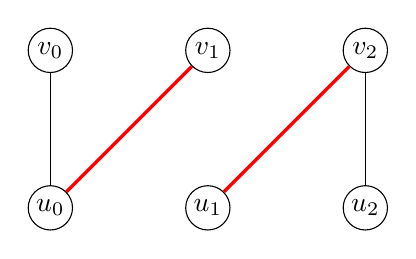
\begin{tikzpicture}[xscale=2,every node/.style={inner sep=0pt, minimum width = 16pt, circle, draw}]
\node (0a) at (0, 0) {$u_0$};
\node (1a) at (1, 0) {$u_1$};
\node (2a) at (2, 0) {$u_2$};
\node (0b) at (0, 2) {$v_0$};
\node (1b) at (1, 2) {$v_1$};
\node (2b) at (2, 2) {$v_2$};
\foreach \x/\y in {0/0, 2/2} 
  \draw (\x a) -- (\y b) ;
\foreach \x/\y in {0/1, 1/2} \draw[very thick, red] (\x a) -- (\y b) ;
\end{tikzpicture}
\end{center}

Dans cet exemple, $C = \{(u_0, v_1), (u_1, v_2)\}$, $U_0 = \{u_2\}$, $Z = \{u_1, v_2\}$ et $T=\{u_0, v_2\}$.

%--------------------------------------------------------------------------
%--------------------------------------------------------------------------
\begin{Exercise}[title=Lemme]\it
Montrer que $T$ est un transversal.
\end{Exercise}
%--------------------------------------------------------------------------
\begin{Answer}
Si $s$ appartient à $Z$ alors il y a un chemin de $x_0$ à $s$ vérifiant
\[x_0 \rightarrow x_1 \rightarrow x_2\rightarrow \cdots \rightarrow x_{p-1} \rightarrow x_p=s\]
\begin{itemize}
    \item $x_0\in U_0$ 
    \item $x_i\in U$ pour $i$ pair, $x_i\in V$ pour $i$ impair, 
    \item $(x_i, x_{i+1})\notin C$ pour $i$ pair, $(x_i, x_{i+1})\in C$ pour $i$ impair. 
\end{itemize}

Si $a = (u, v)$ est une arête du graphe on a
\begin{itemize}
  \item soit $u\in U_0$ donc $(u, v)$ n'est pas une arête du couplage et $v\in Z\cap V \subset T$,
  \item soit $u\in Z\cap U$ donc $u = x_p$ avec $p$ pair et $(x_{p-1}, u)\in C$ ; on en déduit qu'on a
  
  $v = x_{p-1}$ donc $v\in Z\cap V\subset T$
  
  ou $v\ne x_{p-1}$ donc $(u, v)\notin C$ et $v\in Z\cap V \subset T$
  \item Soit $u\in U\setminus(U_0\cup Z)\subset T$.
\end{itemize}

Dans tous les cas une extrémité de l'arête est dans $T$ : $T$ est un transversal.

\end{Answer}
%--------------------------------------------------------------------------
%--------------------------------------------------------------------------
\begin{Exercise}[title=Théorème de König]\it
Montrer que $T$

Montrer que, dans un graphe biparti, $\alpha'(G)=\beta(G)$.
\end{Exercise}
%--------------------------------------------------------------------------
\begin{Answer}
Si $T$ est un transversal, chaque arête d'un couplage a (au moins) une extrémité dans $T$ et les extrémités des arêtes du couplage sont distinctes donc on peut définir une injection de puis l'ensemble des arêtes d'un couplage vers les sommet d'un transversal (en choisissant éventuellement une des deux extrémités). On a donc $|C| \le |T|$ d'où $\alpha'(G) \le \beta(G)$.

\medskip

Pour un couplage maximal $C$, le lemme a construit un transversal $T$.

Tout sommet $u\in T\cap U$ est l'extrémité d'une arête de $C$ car $n\notin U_0$.

Tout sommet $v\in T\cap V$ est l'extrémité d'un chemin alternant commençant par un sommet de $U_0$. S'il n'existait pas d'arête de $C$ passant par $v$, le chemin alternant serait augmentant, ce qui n'est pas possible car $C$ est maximal. $v$ est l'extrémité d'une arête de $C$

Comme il ne peut exister qu'une arête de $C$ passant par un sommet le raisonnement ci-dessus définit une application de $T$ vers $C$.

Si deux sommets distincts étaient associés à une même arête de $C$ on aurait alors $(u, v) \in C$ avec $u\in T$ et $v\in T$. Comme $v\in T\cap V = Z\cap V$, il serait l'extrémité d'un chemin alternant commençant par un sommet de $U_0$ donc $u$ appartiendrait aussi à $Z$, ce qui est impossible car $u\in T\cap U = U\setminus(U_0\cup Z)$.

On a donc une injection de $T$ dans $C$ d'où $|T|\le |C|$ puis $\beta(G) \le \alpha'(G)$.

On en déduit l'égalité souhaitée.
\end{Answer}
%--------------------------------------------------------------------------
%--------------------------------------------------------------------------

On notera $\Gamma(X)$ l'ensemble des sommets adjacents à $X \subset S$.
%--------------------------------------------------------------------------
%--------------------------------------------------------------------------
\begin{Exercise}[title=Théorème de Hall]\it
Montrer qu'un graphe biparti $G$ admet un couplage parfait si et seulement si $|\Gamma(X)| \ge |X|$ pour tout $X\subset U$.
\end{Exercise}
%--------------------------------------------------------------------------
\begin{Answer}
$G = (U\sqcup V, A)$ avec $|U| = |V|=n$.

Si $G$ admet un couplage de cardinal $n$, celui ci définit une bijection $\varphi$ de $U$ vers $V$ donc, pour tout $X\subset U$, $\Gamma(X) \supset \varphi(X)$ et $|\Gamma(X)| \ge |\varphi(X)|=|X|$.

\medskip

On suppose que les inégalités sont vérifiées.

Soit $p$ le cardinal maximal d'un couplage. On a $p\le n$.

D'après le théorème de König, $p$ est le cardinal (minimal) d'un transversal $T$. On note $T_1=T\cap U$ et $T_2=T\cap V$.

Comme $T$ est un transversal, toute arête du graphe a une extrémité dans $T_1$ ou dans $T_2$ donc il n'y a aucune arête allant de $U\setminus T_1$ vers $V\setminus T_2$ ; on a donc $\Gamma(U\setminus T_1) \subset T_2$ et $\Gamma(V\setminus T_2) \subset T_1$. Les inégalités donnent donc

$|V| - |T_2| = |V\setminus T_2| \le |\Gamma(V\setminus T_2)| \le |T_1|$ d'où 
$n \ge |T_1| + |T_2| = p$.

Ainsi $p = n$ et le couplage maximal est parfait.
\end{Answer}
%--------------------------------------------------------------------------
%--------------------------------------------------------------------------
\subsection{Implémentation (Mines 2012)}
%--------------------------------------------------------------------------
%--------------------------------------------------------------------------
$G = (S, A)$ est un graphe biparti équilibré de cardinal $2n$ : $|U| = |V| = n$.

On suppose que les éléments de $U$ et $V$ sont indicées par les entiers de 0 à $n-1$ :
$U = \{u_0, u_1, \ldots, u_{n-1}\}$ et  $V = \{v_0, v_1, \ldots, v_{n-1}\}$.

$G$ est représenté par une matrice de booléens \type{g} de dimension $n\times n$ dont les lignes correspondent aux éléments de $U$ et les colonnes aux éléments de $V$. \type{g.(i).(j)} vaut \type{true} si et seulement si $(u_i, v_j)$ est une arête. 

\begin{center}
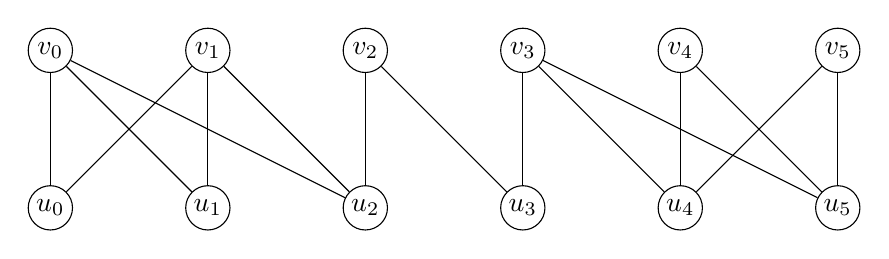
\begin{tikzpicture}[xscale=2,every node/.style={inner sep=0pt, minimum width = 16pt, circle, draw}]
\node (0a) at (0, 0) {$u_0$};
\node (1a) at (1, 0) {$u_1$};
\node (2a) at (2, 0) {$u_2$};
\node (3a) at (3, 0) {$u_3$};
\node (4a) at (4, 0) {$u_4$};
\node (5a) at (5, 0) {$u_5$};
\node (0b) at (0, 2) {$v_0$};
\node (1b) at (1, 2) {$v_1$};
\node (2b) at (2, 2) {$v_2$};
\node (3b) at (3, 2) {$v_3$}; 
\node (4b) at (4, 2) {$v_4$}; 
\node (5b) at (5, 2) {$v_5$}; 
\foreach \x/\y in {0/0, 0/1, 1/0, 1/1, 2/0, 2/1, 2/2, 3/2, 3/3, 4/3, 4/4, 4/5, 5/3, 5/4, 5/5} \draw (\x a) -- (\y b) ;
%\foreach \x/\y in {0/0, 1/1, 3/2, 4/3, 5/5} \draw[very thick, red] (\x a) -- (\y b) ;
\end{tikzpicture}
\end{center}

Le graphe ci-dessus est donc représenté par la matrice :
\begin{lstlisting}
let g = [|[|true;  true;  false; false; false; false|];
          [|true;  true;  false; false; false; false|];
          [|true;  true;  true;  false; false; false|];
          [|false; false; true;  true;  false; false|];
          [|false; false; false; true;  true;  true |];
          [|false; false; false; true;  true;  true |]|];;
\end{lstlisting}
Un couplage $C$ est codé par un tableau d'entiers de taille $n$, \type{c} ; \type{c.(i)} vaut \type{j} si et seulement si $(u_i, v_j)$ est une arête du couplage ou, si $u_i$ n'est pas couplé, \type{c.(i)} vaut \type{-1}.

\type{[|0; 1; -1; 2; 3; 5|]} code le couplage représenté ci-dessous.

\begin{center}
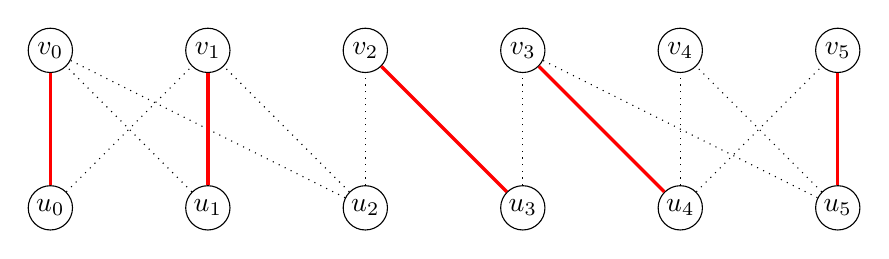
\begin{tikzpicture}[xscale=2,every node/.style={inner sep=0pt, minimum width = 16pt, circle, draw}]
\node (0a) at (0, 0) {$u_0$};
\node (1a) at (1, 0) {$u_1$};
\node (2a) at (2, 0) {$u_2$};
\node (3a) at (3, 0) {$u_3$};
\node (4a) at (4, 0) {$u_4$};
\node (5a) at (5, 0) {$u_5$};
\node (0b) at (0, 2) {$v_0$};
\node (1b) at (1, 2) {$v_1$};
\node (2b) at (2, 2) {$v_2$};
\node (3b) at (3, 2) {$v_3$}; 
\node (4b) at (4, 2) {$v_4$}; 
\node (5b) at (5, 2) {$v_5$}; 
\foreach \x/\y in {0/0, 0/1, 1/0, 1/1, 2/0, 2/1, 2/2, 3/2, 3/3, 4/3, 4/4, 4/5, 5/3, 5/4, 5/5} 
  \draw[dotted] (\x a) -- (\y b) ;
\foreach \x/\y in {0/0, 1/1, 3/2, 4/3, 5/5} \draw[very thick, red] (\x a) -- (\y b) ;
\end{tikzpicture}
\end{center}
%--------------------------------------------------------------------------
%--------------------------------------------------------------------------
\begin{Exercise}[title=]\it
Écrire  une fonction \type{verifie} telle que si \type{g} est une matrice codant le graphe $G$ et \type{c} un tableau codant le couplage $C$ alors \type{verifie g c} renvoie \type{true} si le tableau $C$ représente un couplage dans $G$ et \type{false} sinon.
\end{Exercise}
%--------------------------------------------------------------------------
\begin{Answer}
Pour chaque nouveau couplage rencontré il faut vérifier si l'arête correspondante existe dans le graphe et si elle n'est pas incidente à une arête déjà rencontrée. Pour cela on utilise un tableau \type{vu} qui indique si un sommet de $B$ a déjà été rencontré.
\begin{lstlisting}
let verifie g c =
   let n = Array.length c in
   let reponse = ref true in
   let vu = Array.make n false in
   for i = 0 to (n-1) do
      let j = c.(i) in
      if j <> -1 && not vu.(j)
      then begin reponse := !reponse && g.(i).(j);
           vu.(j) <- true end done;
  !reponse;;
\end{lstlisting}
La complexité est linéaire en $n$, le nombre de sommets.
\end{Answer}
%--------------------------------------------------------------------------
%--------------------------------------------------------------------------
\begin{Exercise}[title=]\it
Écrire  une fonction \type{inverse c} telle que si \type{c} est un tableau codant un couplage $C$ alors \type{inverse c} renvoie tableau \type{inv} codant $C$ depuis $V$ : \type{inv.(j)} vaut \type{i} si $(i, j)$ est une arête du couplage et vaut \type{-1} s'il n'en existe pas.
\end{Exercise}
%--------------------------------------------------------------------------
\begin{Answer}
\begin{lstlisting}
let inverse c = 
   let n = Array.length c in
   let r = Array.make n (-1) in
   for i = 0 to (n-1) do
      if c.(i) <> -1
      then r.(c.(i)) <- i done;
   r;;
\end{lstlisting}
\end{Answer}
%--------------------------------------------------------------------------
%--------------------------------------------------------------------------
\subsection{Recherche exhaustive (Mines 2012)}
%--------------------------------------------------------------------------
%--------------------------------------------------------------------------
\begin{Exercise}[title=]\it
Écrire une fonction \type{une\_arete g} qui renvoie une arête quelconque du graphe représenté par \type{g} sous la forme \type{Some (u, v)} s'il existe au moins une arête $(u, v)$, sinon la fonction renvoie  \type{None}.
\end{Exercise}
%--------------------------------------------------------------------------
\begin{Answer}
\begin{lstlisting}
let une_arete g =
   let n = Array.length g in
   let out = ref None in
   for u = 0 to (n-1) do
      for v = 0 to (n-1) do
         if g.(u).(v) then out := Some (u, v) done done;
   !out;;
\end{lstlisting}
\end{Answer}
%--------------------------------------------------------------------------
%--------------------------------------------------------------------------
On cherche un algorithme qui permette de déterminer un couplage de cardinal maximal dans un graphe biparti équilibré ; le principe est le suivant.

Si le graphe courant ne contient aucune arête, le cardinal maximum d'un couplage est 0 et aucun sommet n'est couplé.

Dans le cas contraire, l'algorithme considère une arête quelconque $a$ du graphe courant et recherche successivement :
\begin{itemize}
  \item un couplage de cardinal maximal parmi les couplages du graphe courant ne contenant pas $a$ ;
  \item un couplage de cardinal maximal parmi les couplages du graphes contenant $a$.
\end{itemize}
L'algorithme déduit alors un couplage de cardinal maximal.
%--------------------------------------------------------------------------
%--------------------------------------------------------------------------
\begin{Exercise}[title=]\it
Écrire une fonction \type{copie\_matrice} qui copie une matrice. 

On pourra utiliser la fonction \type{Array.copy} qui copie un tableau mais ne permet pas de copier une matrice en assurant que les valeurs de chaque ligne soient indépendantes de la matrice originale.
\end{Exercise}
%--------------------------------------------------------------------------
\begin{Answer}
\begin{lstlisting}
let copie_matrice m = 
   let n = Array.length m in
   let cop = Array.make n [||] in
   for i = 0 to (n-1) do
      cop.(i) <- Array.copy m.(i) done;
   cop;;
\end{lstlisting}
\newpage
\end{Answer}
%--------------------------------------------------------------------------
%--------------------------------------------------------------------------
\begin{Exercise}[title=]\it
Écrire une fonction \type{meilleur\_couplage g} qui renvoie un tableau codant un couplage de cardinal maximal dans $G$.
\end{Exercise}
%--------------------------------------------------------------------------
\begin{Answer}
Pour ne pas avoir à compter la taille du couplage, on renvoie celle-ci dans une fonction auxiliaire en plus du couplage. Pour déterminer un couplage auquel on pourra ajouter une arête $a=(u, v)$, on part du graphe qui interdit toute arête depuis $u$ ou vers $v$.
\begin{lstlisting}
let rec meilleur_couplage g =
   let n = Array.length g in
   let rec aux_mc g =
     match une_arete g with
     |None -> Array.make n (-1), 0
     |Some (u, v) ->  let g1 = copie_matrice g in
                      g1.(u).(v) <- false;
                      let g2 = copie_matrice g in
                      for k = 0 to (n-1) do
                         g2.(u).(k) <- false;
                         g2.(k).(v) <- false done;
                      let c1, n1 = aux_mc g1 in
                      let c2, n2 = aux_mc g2 in
                      c2.(u) <- v;
                      if n1 > n2 then c1, n1 else c2, (n2+1)
   in aux_mc g;;
\end{lstlisting}
Les complexités temporelles et spatiales sont monstrueuses : de l'ordre de $n^2.2^{n^2}$.
\end{Answer}
%--------------------------------------------------------------------------
\newpage
%--------------------------------------------------------------------------
\subsection{Algorithme Hongrois (Mines 2012)}
%--------------------------------------------------------------------------
%--------------------------------------------------------------------------
L'{\bf algorithme hongrois} s'appuie sur le théorème de Berge et détermine un couplage de cardinal maximal dans $G$. L'algorithme débute avec un couplage $C$ de cardinal nul ; tant qu'il existe une chaîne augmentante relativement à $C$, l'algorithme modifie $C$ pour incrémenter de 1 le cardinal du couplage en utilisant une telle chaîne augmentante.

Pour trouver une chaîne alternée augmentante, on recherche les sommets qui sont extrémités de chaînes alternées en procédant de proche en proche à partir des sommets de $A$ non couplés.

Un sommet $y$ est dit {\bf atteint} si une chaîne alternée relativement à $C$ et d'extrémité $y$ est mise en évidence. 

Au départ tous les sommets non couplés de $U$ (un tel sommet est extrémité d'une chaîne alternée réduite à ce sommet) sont considérés comme atteints ; aucun autre sommet n'est considéré comme atteint. Un sommet $y$ non encore atteint peut être atteint à partir d'un de ses voisins $x$ {\bf déjà atteint} si on a :
\begin{itemize}
  \item soit $y$ est dans $V$ (et donc $x$ est dans $A$) et l'arête $(x,y)$ n'est pas dans le couplage $C$ ;
  \item soit $y$ est dans $U$ (et donc $x$ est dans $V$) et l'arête $(y, x)$ est dans le couplage $C$.
\end{itemize}

On utilise des marques attribuées aux sommets. Ces marques sont des entiers initialisés à $-1$ pour tous les sommets. Lorsqu'un sommet $y$ est atteint à partir d'un sommet $x$ la marque de $y$ devient égale au numéro de $x$ (on rappelle que le numéro d'un sommet $u_i$ ou $v_i$ vaut $i$) ; $x$ est alors l'avant-dernier sommet dans la chaîne alternée Ch$(y)$ d'extrémité $y$ mise en évidence. La chaîne Ch$(y)$ peut être retrouvée à l'envers, de proche en proche, grâce aux marques ; dans cette chaîne, seule l'origine porte une marque de valeur $-1$. Si un sommet non couplé $y$ de $V$ est atteint, Ch$(y)$ est une chaîne alternée augmentante relativement à $C$.

On pourra utiliser définir deux fonctions \type{chercherU} et \type{chercherV} utilisant une récursivité croisée (chacune pouvant appeler l'autre) telles que telle que \type{chercherX s} détermine des sommets non encore atteints qui peuvent être atteints, de voisin en voisin, récursivement, à partir de $s\in X$ en modifiant les marques de ces sommets nouvellement atteints et s’arrête dans les cas suivants :
\begin{itemize}
    \item un sommet $v_i\in V$ non couplé a été atteint ; elle renvoie alors $i$
    \item tous les sommets qui peuvent être atteints de voisin en voisin à partir de $s$ l’ont
été et aucun sommet non couplé de $V$ n’est atteint ; elle renvoie alors $-1$.
\end{itemize}

%--------------------------------------------------------------------------
%--------------------------------------------------------------------------
\begin{Exercise}[title=]\it
Écrire une fonction \type{chaine\_augmentante g c} qui renvoie un triplet formé de deux tableaux codant les marques d'une chaîne alternée augmentante du graphe $G$ pour le couplage $C$ et le numéro de l'extrémité (dans $V$) de ce couplage.

S'il n'existe pas de chaîne alternée augmentante le numéro sera \type{-1}.
\end{Exercise}
%--------------------------------------------------------------------------
\begin{Answer}
On parcourt dans l'ordre les sommets de $A$ jusqu'à trouver un éventuel sommet non couplé origine d'une chaîne alternée augmentante. 

\begin{lstlisting}
let chaine_augmentante g c =
   let n = Array.length c in
   let r = inverse c in
   let fin  = ref (-1) in
   let mU = Array.make n (-1) in
   let mV = Array.make n (-1) in
   let rec chercherU u =
   (* on cherche les sommets atteignables non vus et non couplés à u *)
      let v = ref 0 in
      while !v < n && !fin = -1 do         
         if g.(u).(!v) && c.(u) <> !v && mV.(u) = -1 
         then begin mV.(!v) <- u;
              chercherV !v;
              if !fin = -1 then mV.(!v) <- -1 end;
         v := !v + 1 done;
   and chercherV v = 
      match r.(v) with
      |(-1) -> fin := v
      |u -> mU.(u) <- v;
            chercherU u in
   let u = ref 0 in
   while !u < n && !fin = -1 do
      for k = 0 to (n-1) do mU.(k) <- -1; mV.(k) <- -1 done;
      chercherU !u;
      u := !u + 1 done;
   mU, mV, !fin;;
\end{lstlisting}
\newpage
\end{Answer}
%--------------------------------------------------------------------------
%--------------------------------------------------------------------------
\begin{Exercise}[title=]\it
Écrire une fonction \type{actualiser c mU mV fin} qui modifie le couplage codé par $c$ en utilisant la chaîne alternée augmentante codée par les tableaux \type{mU} et \type{mV} et le sommet final \type{fin}.
\end{Exercise}
%--------------------------------------------------------------------------
\begin{Answer}

On remonte la chaîne augmentante grâce aux marques en partant de \type{fin} ; 

pour un sommet $v$ de $V$,  on lit \type{u = mB.(v)} et on crée l'arête $(u, v)$ dans le couplage 

puis on recommence à partir de \type{mU.(u)} s'il est distinct de $-1$.
\begin{lstlisting}
let actualiser c mU mV fin =
   let rec actu v =
       let u = mV.(v) in
       c.(u) <- v;
       let v1 = mU.(u) in
       if v1 <> -1 then actu v1 in
   actu fin;;
\end{lstlisting}
\end{Answer}
%--------------------------------------------------------------------------
%--------------------------------------------------------------------------
\begin{Exercise}[title=]\it
Écrire une fonction \type{algorithme\_hongrois g} qui renvoie un tableau codant un couplage de cardinal maximal dans $G$ en utilisant cette méthode.
\end{Exercise}
%--------------------------------------------------------------------------
\begin{Answer}
\begin{lstlisting}
let algorithme_hongrois g = 
   let n = Array.length g in
   let c = Array.make n (-1) in
   let rec aux_hon () =
      let mU, mV, fin  = chaine_augmentante g c in
      if fin = -1 
      then c
      else begin actualiser c mU mV fin;
                 aux_hon () end in
   aux_hon ();;
\end{lstlisting}
\end{Answer}
%--------------------------------------------------------------------------
%--------------------------------------------------------------------------
